

\paragraph{Sigmoid}

\begin{align}
sigmoid(x)&= \frac{1}{1+e^{-x}}  \\ 
sigmoid'(x)&= sigmoid(x) \cdot (1-sigmoid(x))
\end{align}

As we can see from figure \ref{sigmoid_plot}, the sigmoid derivative has only one maximum in 0 where it assume value 0.25. Receding from 0, in both direction leads to regions where
the the derivative take zero value, such regions are called \textit{saturation} regions. If we happen to be in such regions, for a given neuron, we cannot learn anything since that neuron doesn't contribute
to the gradient.

\begin{figure}[h]
  \centering
    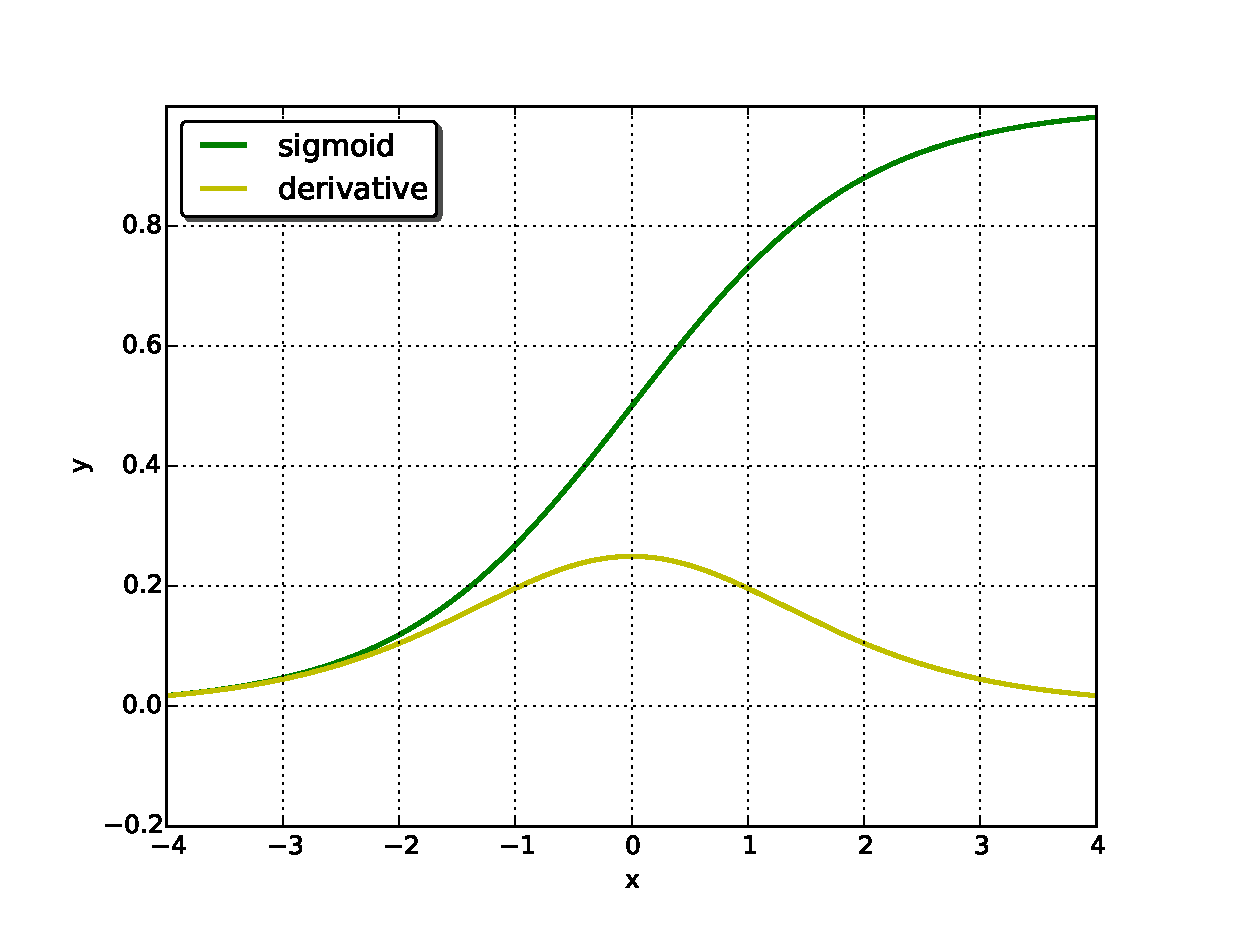
\includegraphics[width=0.9\textwidth]{sigmoid_and_deriv.eps}
  \caption{sigmoid and it's derivative}
\label{sigmoid_plot}
\end{figure}



\paragraph{ReLU}


\begin{align}
  ReLU(x)&=\begin{cases}
    x & \text{if $x>0$}.\\
    0 & \text{otherwise}.
  \end{cases} \\ 
   ReLU'(x)&=\begin{cases}
    1 & \text{if $x>0$}.\\
    0 & \text{otherwise}.
  \end{cases}
\end{align}


As we can see from figure \ref{relu_plot}, ReLU's derivative is a step function; it has only one \textit{saturation} region $(-\inf, 0]$ and a region in which is always takes value one, $(0,+\inf]$
This leads to the fact that we cannot learn to 'turn on' a swictched off neuron ($x<0$), but we have no \textit{saturation} region toward $+\inf$.

\begin{figure}[h]
  \centering
    \includegraphics[width=0.9\textwidth]{relu_and_deriv.eps}
  \caption{ReLU and it's derivative}
\label{relu_plot}
\end{figure}
